 \documentclass[a4paper, 11pt]{article}
\usepackage{comment} % enables the use of multi-line comments (\ifx \fi)
\usepackage{lipsum} %This package just generates Lorem Ipsum filler text.
\usepackage{fullpage} % changes the margin
\usepackage{indentfirst}
\usepackage{graphicx}
\usepackage{amsmath}

\begin{document}
%Header-Make sure you update this information!!!!
\noindent
\large\textbf{Report: Computer Graphics} \hfill \textbf{Xucheng Chen} \\
\normalsize COMS 4160 \hfill xc2360 \\
Prof. Zheng \hfill Date: 02/23/2017

\section*{Running the code}
    \indent I basically finished all coding in eclipse, so the easiest way to compile and run the code would be just import the code in eclipse and then configure the build path to include the lwjgl library. After importing the project, just run Main.java:). If you have any  problems running the sample code, please contact me and I will personally demo it in office hours.

\section*{User Manual}
    There are two different rendering modes that user can choose: 3D and 2D, just simply change the SceneType st in Main.java file to whichever mode you prefer.
    \subsection{2D Forward Kinematics}
        \begin{center}
            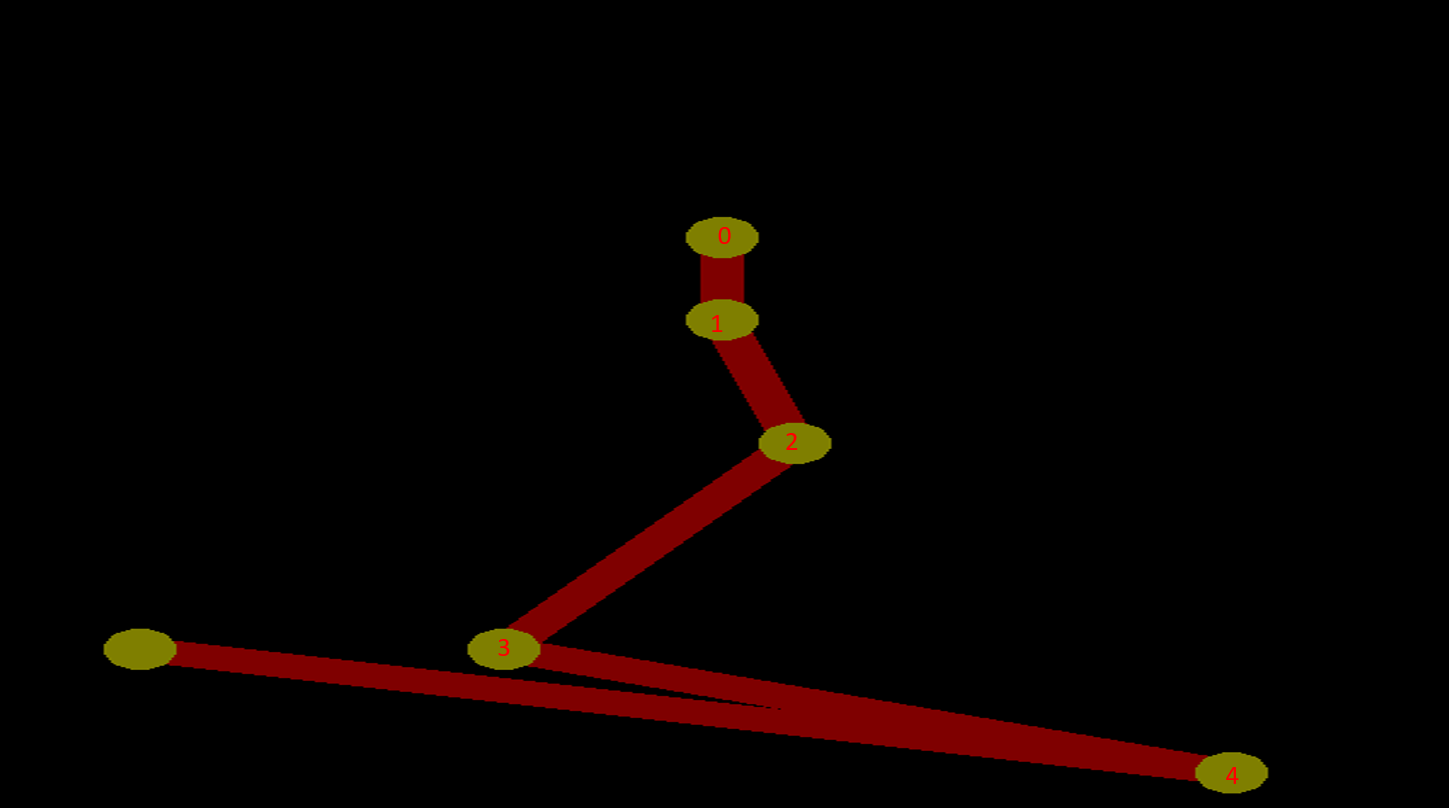
\includegraphics[width = \textwidth]{Capture0.PNG}
        \end{center}
        The basic control keys are listed below:(increase means change the angle in counter-clockwise way, decrease means change the angle in clockwise way)
        \begin{itemize}
            \item A: Increase the rotation angle of joint 1
            \item S: Increase the rotation angle of joint 2
            \item D: Increase the rotation angle of joint 3
            \item F: Increase the rotation angle of joint 4
            \item Z: Decrease the rotation angle of joint 1
            \item X: Decrease the rotation angle of joint 2
            \item C: Decrease the rotation angle of joint 3
            \item V: Decrease the rotation angle of joint 4
        \end{itemize}

    \subsection{2D Inverse Kinematics}
        \begin{center}
            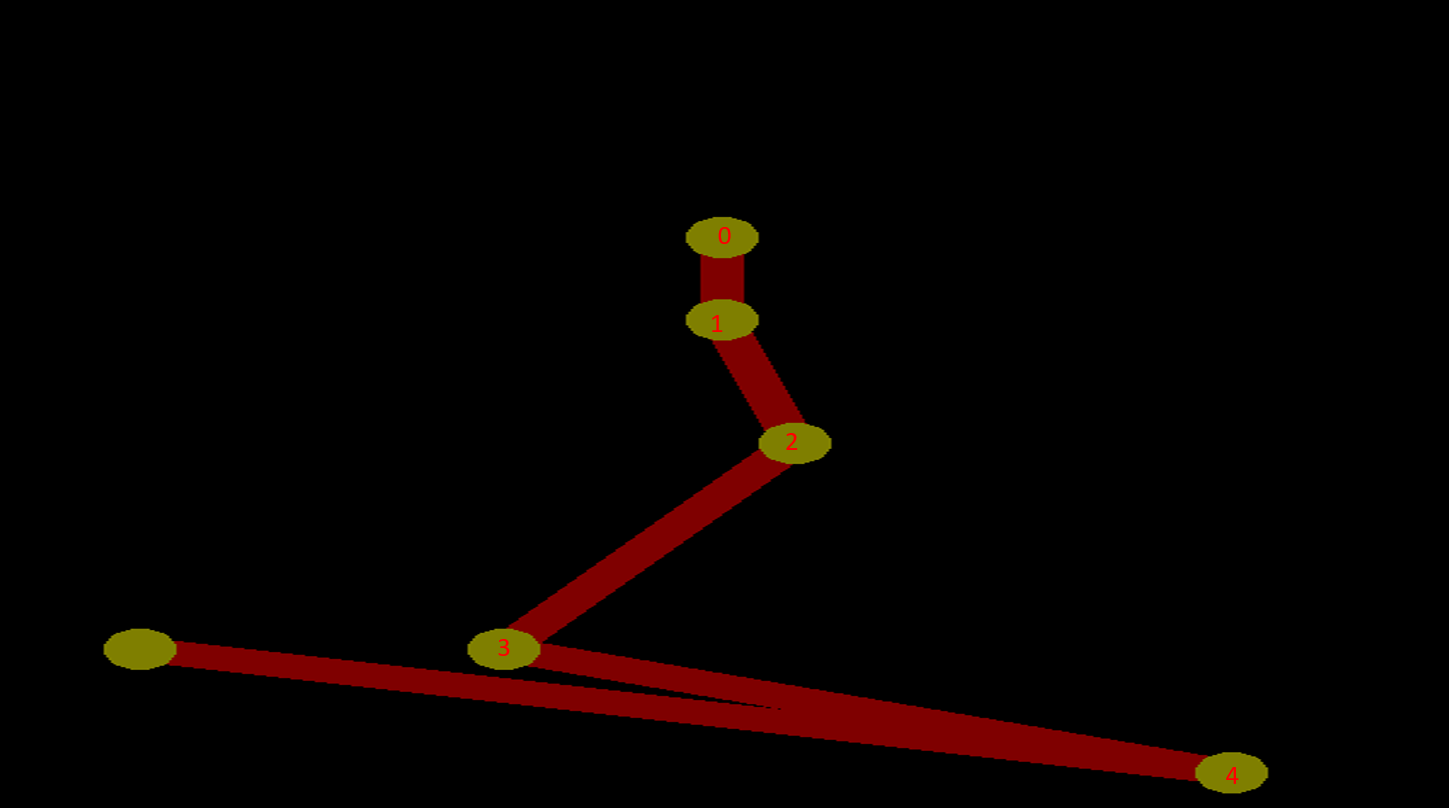
\includegraphics[width = \textwidth]{Capture0.PNG}
        \end{center}
        In 2D inverse kinematics, just simply click any joints and dray it to wherever you want it to be.
    \subsection{3D Forward Kinematics}
        There are two shapes that users can choose, one is a simple arm, and the other is a rather complex puppy. To choose from these two shapes, just change the file to be read(puppy.xml for puppy, object.xml for simple arm). Also, in order to see the 3D effect, I add three axis in the scene: red for z-axis, blue for x-axis and green for y-axis. I have basically abandoned all codes given by TA in 3D kinematics, and have rewritten them based on the previous assignments. So users can click left mouse button and dray to change the view of camera.
        \begin{center}
            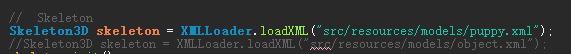
\includegraphics[width = \textwidth]{Capture2.PNG}
        \end{center}

        \begin{center}
            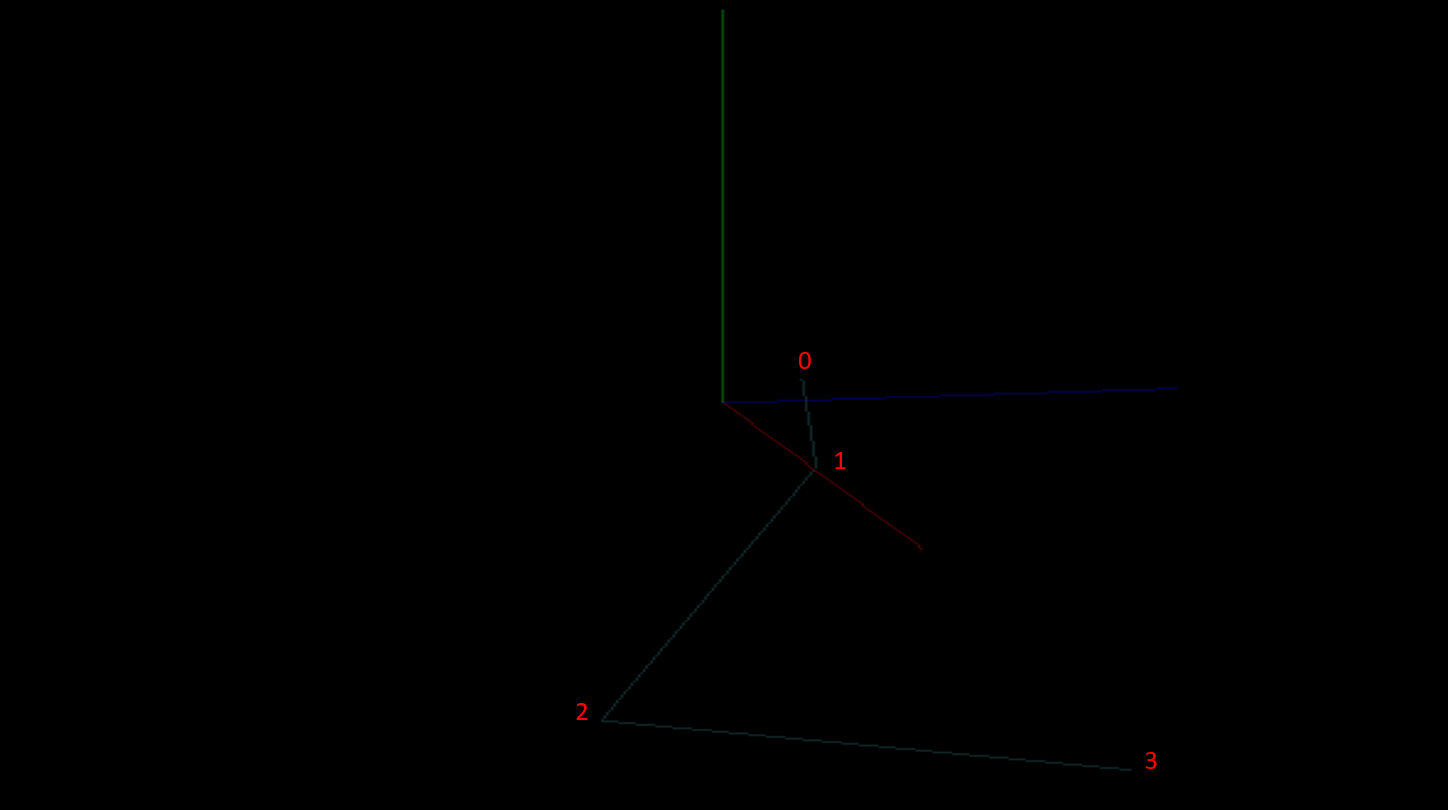
\includegraphics[width = \textwidth]{Capture5.PNG}
        \end{center}
        In 3D kinematics, I am using spherical coordinate system, each joint has two rotation angles theta and phi(see the graph).
        \begin{center}
            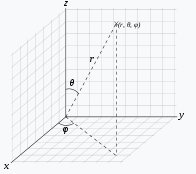
\includegraphics[width = .6\textwidth]{Capture4.PNG}
        \end{center}
        \begin{itemize}
            \item Z: Increase the rotation angle phi of arm 2-3 by 1 degree
            \item X: Increase the rotation angle theta of arm 2-3 by 1 degree
            \item E: Increase the rotation angle phi of arm 0-1 by 1 degree
            \item R: Increase the rotation angle theta of arm 0-1 by 1 degree
            \item T: Increase the rotation angle phi of arm 1-2 by 1 degree
            \item Y: Increase the rotation angle theta of arm 1-2 by 1 degree
        \end{itemize}

    \subsection{3D Inverse Kinematics}
        In addition, I have implemented a 3D inverse kinematics, user can click right mouse button and drag the joint to whichever position they want. However, the 3D inverse kinematics does not work well with structures with joints of same x and y coordinates but different z coordinates. For example, if the structure has joint (0,0,1) and (0,0,0.5), the 3D inverse kinematics I implemented can only select the latter.
    \subsection{3D Animation}
        The basic control keys are listed below:
        \begin{itemize}
          \item B: Select key frames
          \item N: Start rendering animation
          \item M: Resume selecting key frames stage
        \end{itemize}
        Once you select like 3 poses by pressing B three times, you can press N to see the animation, which will loop non-stoppingly on the screen. Once you are tired of it, just press M to resume the stage of selecting key frames.
        \subsubsection{Simple arm}
            The following shows the key frames:(sequential order)
            \begin{center}
                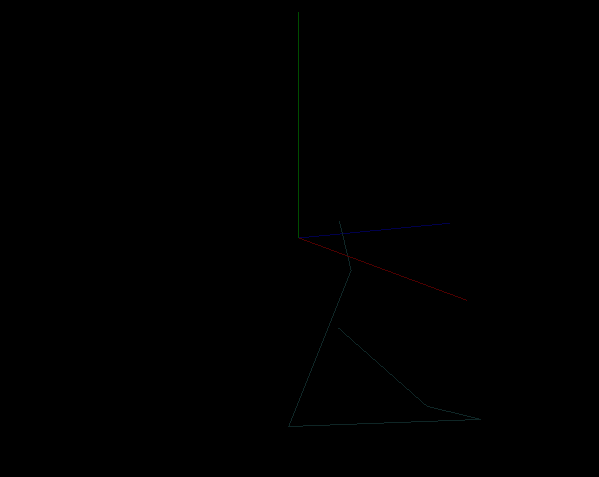
\includegraphics[width = \textwidth]{Animation1-1.PNG}
            \end{center}
            \begin{center}
                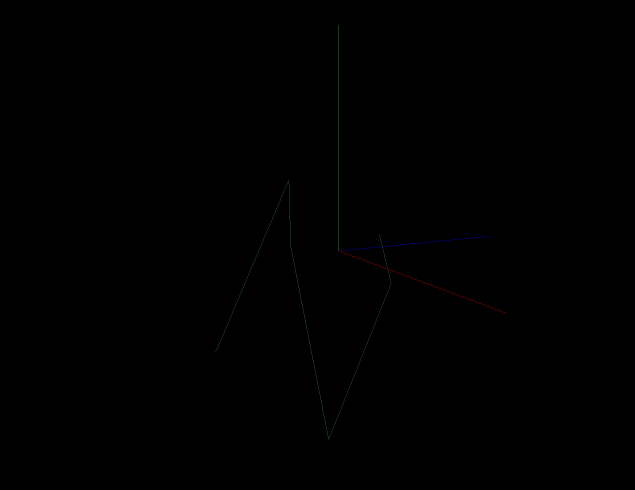
\includegraphics[width = \textwidth]{Animation1-2.PNG}
            \end{center}
            \begin{center}
                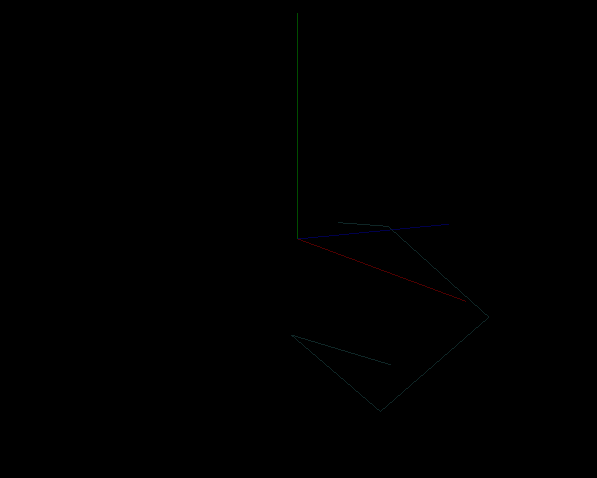
\includegraphics[width = \textwidth]{Animation1-3.PNG}
            \end{center}
            \begin{center}
                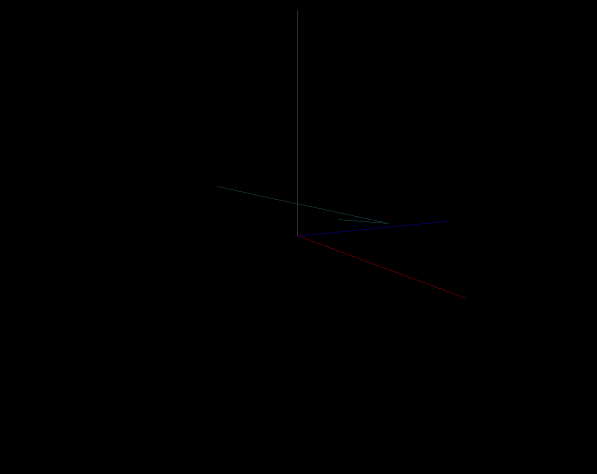
\includegraphics[width = \textwidth]{Animation1-4.PNG}
            \end{center}
            \begin{center}
                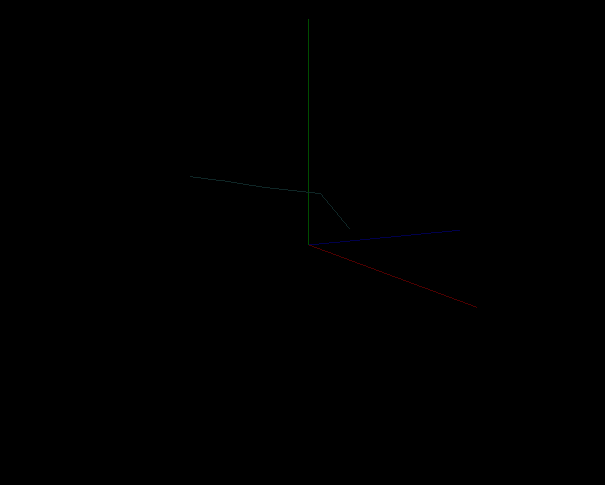
\includegraphics[width = \textwidth]{Animation1-5.PNG}
            \end{center}

        \subsubsection{Puppy}
            The following shows the key frames:(sequential order)
            \begin{center}
                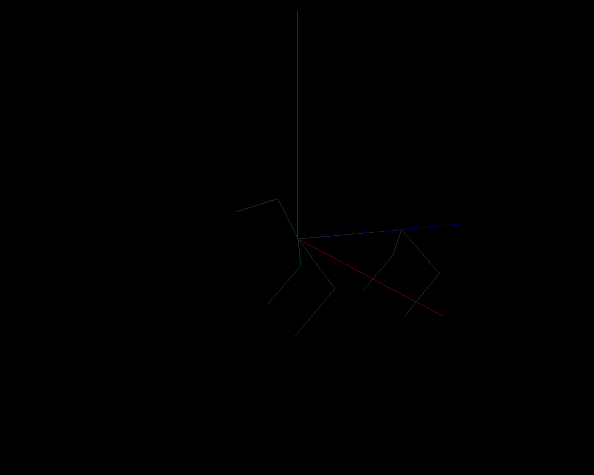
\includegraphics[width = \textwidth]{Animation2-1.PNG}
            \end{center}
            \begin{center}
                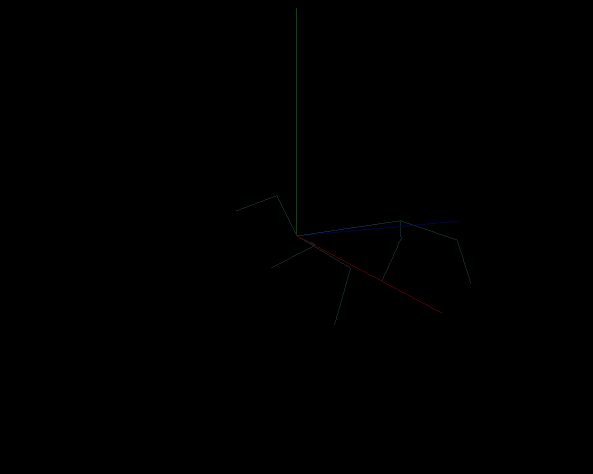
\includegraphics[width = \textwidth]{Animation2-2.PNG}
            \end{center}
            \begin{center}
                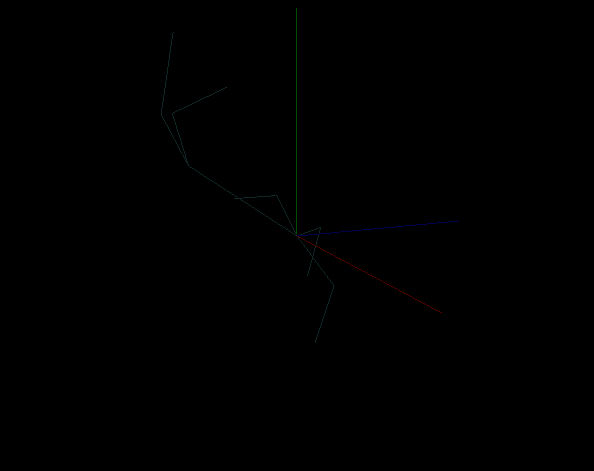
\includegraphics[width = \textwidth]{Animation2-3.PNG}
            \end{center}
            \begin{center}
                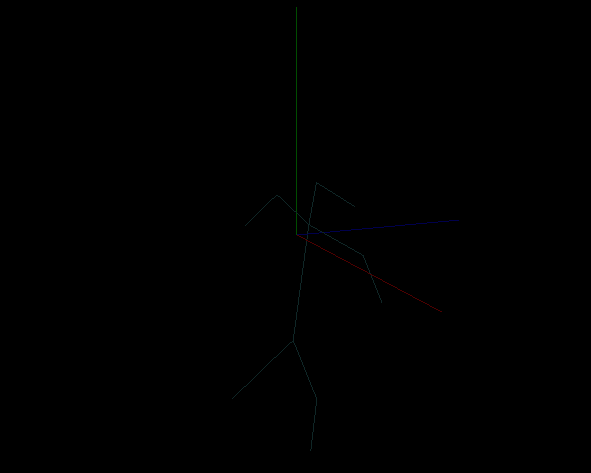
\includegraphics[width = \textwidth]{Animation2-4.PNG}
            \end{center}
            \begin{center}
                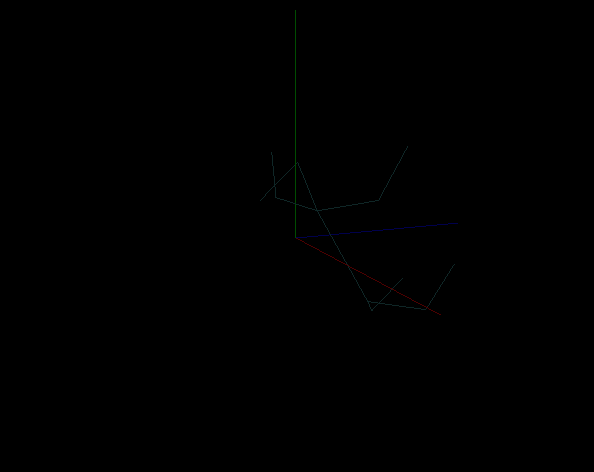
\includegraphics[width = \textwidth]{Animation2-5.PNG}
            \end{center}

\section*{Installiation}
   \indent The following installation guide is copied from the official website of lwjgl: Eclipse supports Gradle/Maven projects and it is highly recommended to use them instead of a manual Eclipse project configuration. However, if you prefer setting up a native Eclipse project, follow these instructions (works with Eclipse Neon):

\begin{itemize}
   \item     Download the ZIP bundle from https://www.lwjgl.org/download
   \item     When the download is complete, extract its contents to some file system directory, henceforth referred to as <lwjgl3>.
   \item     In Eclipse go to menu "Window" > "Preferences" and in the tree view to the left search for 'Java' > 'Build Path' > 'User Libraries' and Click "New..." in the 'User Libraries' dialog. In the opened modal dialog "New User Library" write "LWJGL3" in the 'User library name:' text field and click 'OK'. The newly created library "LWJGL3" should show up in the list 'Defined user libraries:'.
   \item     Now, select this item in the list and click 'Add External JARs...'. This opens a standard OS file selection dialog allowing you to select *.jar files which get added to the classpath/buildpath of all projects using the LWJGL3 User Library. Go to <lwjgl3> and select all *.jar files which do not have -javadoc or -sources in their names. Make sure you don't forget the lwjgl-natives-<os>.jar file, and click 'Open'. This will populate the LWJGL3 user library in the list with respective entries for all selected jar files. You could leave it at that now in order to use LWJGL 3.
   \item     However, if you want to have Sources and JavaDocs, you will have to select each of the entries, click on 'Source attachment: (None)' and on 'Edit...'. This will open the "Source Attachment Configuration" dialog. Here you could select 'External location' and 'External File...' to select the appropriate *-sources.jar file.
   \item     In order to actually use the LWJGL3 User Library in one of your projects, go to the Build Path settings of your project and select the 'Libraries' tab. Here, click 'Add Library...', select 'User Library' and mark the "LWJGL3" User Library.
   \item     Now you are set up to use LWJGL 3 in your project.
\end{itemize}

% to comment sections out, use the command \ifx and \fi. Use this technique when writing your pre lab. For example, to comment something out I would do:
%  \ifx
%   \begin{itemize}
%       \item item1
%       \item item2
%   \end{itemize}
%  \fi

\ifx

\section*{Attachments}
%Make sure to change these
Lab Notes, HelloWorld.ic, FooBar.ic
%\fi %comment me out

\begin{thebibliography}{9}
\bibitem{Robotics} Fred G. Martin \emph{Robotics Explorations: A Hands-On Introduction to Engineering}. New Jersey: Prentice Hall.
\bibitem{Flueck}  Flueck, Alexander J. 2005. \emph{ECE 100}[online]. Chicago: Illinois Institute of Technology, Electrical and Computer Engineering Department, 2005 [cited 30
August 2005]. Available from World Wide Web: (http://www.ece.iit.edu/~flueck/ece100).
\end{thebibliography}
\fi
\end{document} 